\section{问题一：典型日循环优化}

\subsection{确定性线性规划}

问题一的负荷、光伏和电价均已知，且不允许应急购电。令购电价格为 $c_t$，主目标为
\begin{equation}
 \min\ C_1=\sum_{t=0}^{143}c_tg_t,
 \label{eq:q1objective}
\end{equation}
并在式\eqref{eq:balance}--\eqref{eq:bounds}基础上增加 $u_t=0$、$S_0=S_{144}=6000$。该模型是线性规划。由于同一最优费用下可能存在多种等价储能轨迹，先求得最小费用 $C_1^*$，再在
\begin{equation}
 C_1\le C_1^*+10^{-8}\max\{1,|C_1^*|\}
 \label{eq:q1tol}
\end{equation}
的容差内最小化 $\sum_t(x_t+y_t)$。因此，报告的费用具有主目标最优性，而储能轨迹是低吞吐代表解，不宣称是唯一最优轨迹。

\subsection{调度结果}

求解得到总购电量 $59482.698167\,\mathrm{kWh}$，现金费用 $35126.948941$ 元；全天充电量和放电量分别为 $20740.661758$ 与 $16799.936024\,\mathrm{kWh}$，弃光为0。初末SOC均为 $6000\,\mathrm{kWh}$，全天最小与最大SOC恰为 $1200$ 和 $10800\,\mathrm{kWh}$。逐槽母线平衡最大绝对残差为 $9.10\times10^{-13}\,\mathrm{kWh}$。

图\ref{fig:q1-schedule}显示储能在低价时段吸收外购电或光伏，在高价时段放电。由于单向效率为0.9，只有足够大的价差才能覆盖往返损耗；约束边界处的平段说明容量而非价格判断成为局部瓶颈。日末恢复6000 kWh保证该典型日策略不通过透支期末电量来虚降费用。

\begin{figure}[H]
  \centering
  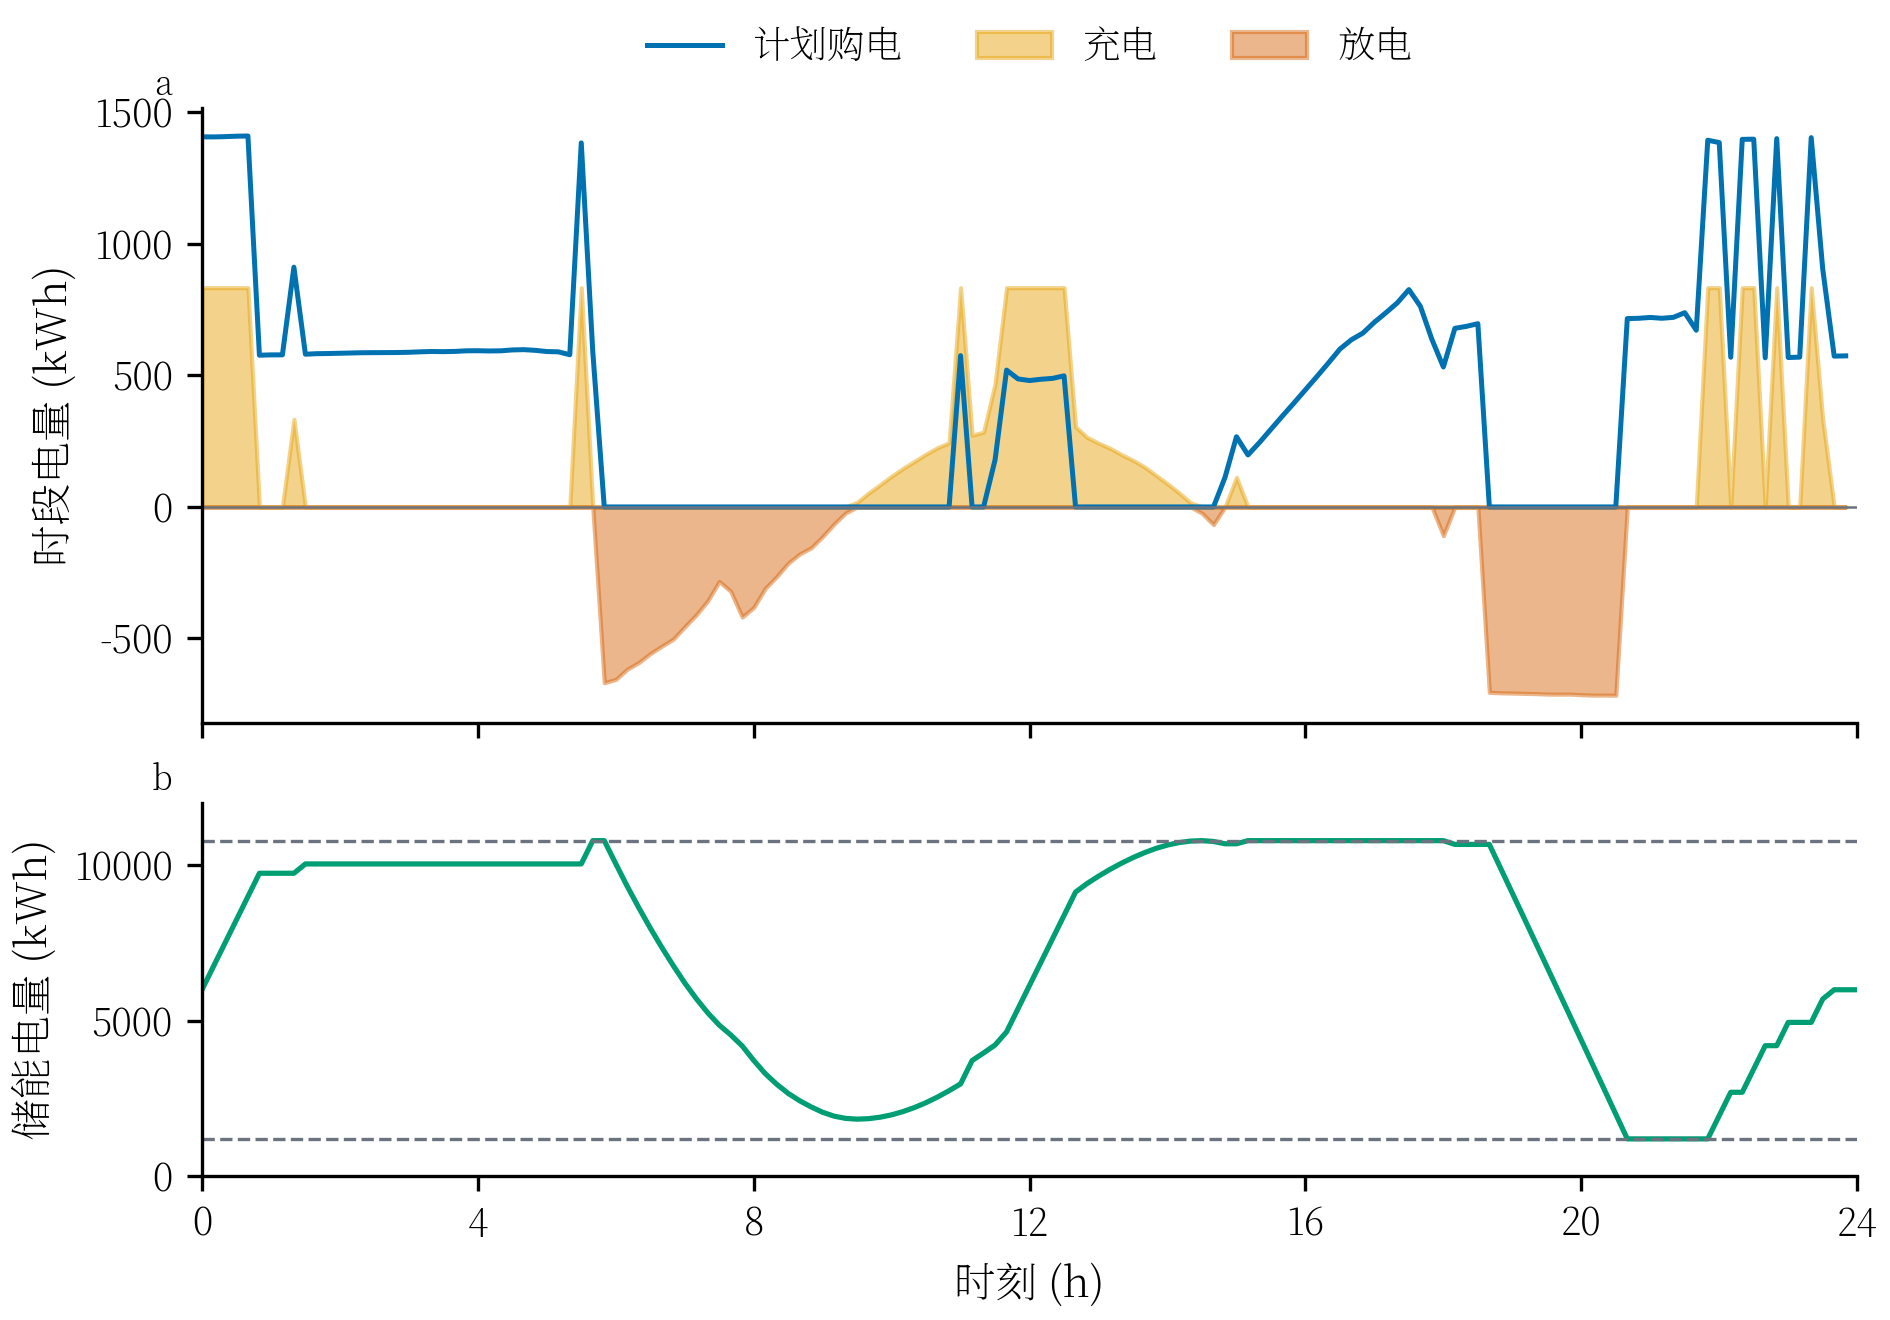
\includegraphics[width=0.97\textwidth]{figs/result_q1_optimal_schedule.png}
  \caption{问题一最优购电、充放电与SOC轨迹。SOC序列含0时和24时两个边界点。}
  \label{fig:q1-schedule}
\end{figure}

题目指定的六个10分钟购电量列于表\ref{tab:q1purchase}。其中12:00、16:00和18:00时起始槽需要购电，而10:00、14:00和20:00时起始槽购电为0。这里每个数值对应单个10分钟槽，不是整小时电量。

\begin{table}[H]
\centering
\caption{问题一指定时段购电量}
\label{tab:q1purchase}
\resizebox{\textwidth}{!}{%
\begin{tabular}{ccccccc}
\toprule
自然区间 & 10:00--10:10 & 12:00--12:10 & 14:00--14:10 & 16:00--16:10 & 18:00--18:10 & 20:00--20:10\\
\midrule
购电量/kWh & 0 & 480.41245 & 0 & 445.43165 & 531.89405 & 0\\
\bottomrule
\end{tabular}}
\end{table}

四小时聚合结果见表\ref{tab:q1battery}。充电量和放电量均由对应24个10分钟槽求和，SOC则取自然0时和24时边界。

\begin{table}[H]
\centering
\caption{问题一各4小时储能电量}
\label{tab:q1battery}
\begin{tabular}{crr@{\qquad}crr}
\toprule
时段 & 充电/kWh & 放电/kWh & 时段 & 充电/kWh & 放电/kWh\\
\midrule
0--4时 & 4500.000 & 0.000 & 12--16时 & 5286.035 & 91.101\\
4--8时 & 833.333 & 6365.838 & 16--20时 & 0.000 & 5780.132\\
8--12时 & 4787.960 & 1702.997 & 20--24时 & 5333.333 & 2859.868\\
\midrule
\multicolumn{3}{c}{0时SOC：6000 kWh} & \multicolumn{3}{c}{24时SOC：6000 kWh}\\
\bottomrule
\end{tabular}
\end{table}

若把全部标签整体解释为区间起点并循环平移10分钟，购电量几乎不变，而费用变为 $35126.848941$ 元，比主口径低约0.10元。这说明时间映射对总量稳健，但费用并非严格不变，故仍应统一自然区间定义。
